\documentclass[preview]{standalone}
\usepackage{tikz}
\usetikzlibrary{calc}
\usepackage{xcolor}
\definecolor{tordion}{RGB}{0,0,255}
\definecolor{agraviton}{RGB}{255,0,0}
\definecolor{sgraviton}{RGB}{0,255,0}
\begin{document}
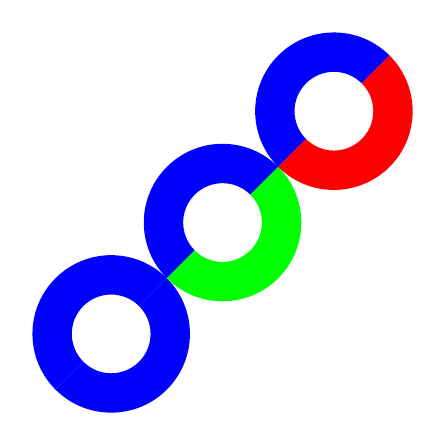
\begin{tikzpicture}[node distance = 1.4cm, auto]
\clip (225:1.5) rectangle (45:5.5);
\coordinate (gauge0) at (45:0);
\fill[tordion] ($(gauge0)+(45:1)$) arc (45:225:1) -- ($(gauge0)+(225:0.5)$) -- ($(gauge0)+(225:0.5)$) arc (225:45:0.5) -- cycle;
\fill[tordion] ($(gauge0)+(-135:1)$) arc (-135:45:1) -- ($(gauge0)+(45:0.5)$) -- ($(gauge0)+(45:0.5)$) arc (45:-135:0.5) -- cycle;
\coordinate (gauge1) at (45:2);
\fill[tordion] ($(gauge1)+(45:1)$) arc (45:225:1) -- ($(gauge1)+(225:0.5)$) -- ($(gauge1)+(225:0.5)$) arc (225:45:0.5) -- cycle;
\fill[sgraviton] ($(gauge1)+(-135:1)$) arc (-135:45:1) -- ($(gauge1)+(45:0.5)$) -- ($(gauge1)+(45:0.5)$) arc (45:-135:0.5) -- cycle;
\coordinate (gauge2) at (45:4);
\fill[tordion] ($(gauge2)+(45:1)$) arc (45:225:1) -- ($(gauge2)+(225:0.5)$) -- ($(gauge2)+(225:0.5)$) arc (225:45:0.5) -- cycle;
\fill[agraviton] ($(gauge2)+(-135:1)$) arc (-135:45:1) -- ($(gauge2)+(45:0.5)$) -- ($(gauge2)+(45:0.5)$) arc (45:-135:0.5) -- cycle;
\end{tikzpicture}
\end{document}
